\noindent
%\vspace{-8mm}
\subsection{Comparison of different broadcast strategies on gnutella Topology}
%\vspace{-4mm}
% We measure 
% the performance of the four algorithms (B-P, X-P-P, P-G and P-P-G) on three real network traces based on broadcast time, 
% wastage and coverage. The data sets are Gnutella network snapshots namely 
% p2p-Gnutella04 (gnutella1), p2p-Gnutella06 (gnutella2) and p2p-Gnutella25 (gnutella3) ~\cite{leskovec2007graph,ripeanu2002mapping} taken on dates August 4, August 6 and August 25, 2002 respectively. 
% The gnutella1 network has 10876 nodes and 39994 edges in its largest connected component. Corresponding number of nodes and edges in the largest connected component 
% in gnutella2 and gnutella3 are respectively 8717, 31525 and 22663, 54693. We simulate these algorithms for varying message sizes.
% We perform our simulations on peer-to-peer systems specifically as our study can find a major application in such systems.

% For simulating the X-P-P algorithm in particular we first need to obtain the best value of x for each network and then run the simulations for varying message sizes. 
%  In figure ~\ref{ps_bt} and ~\ref{ps_wa}, we show how the broadcast time and wastage varies with x for gnutella1 network. We observe that the best value of x lies around 
%  50\%. Similarly we obtained the value of x for the other two datasets as well and found it to be around 50\% and 60\% for gnutella2 and gnutella3 
%  respectively.
% \begin{figure}
% \centering
% \includegraphics[scale=0.15]{figs1/xperbt.eps}
% \includegraphics[scale=0.15]{figs1/xperwa.eps}
% \caption{Average broadcast time and wastage versus x for gnutella1,gnutella2 and gnutella3\vspace{-5mm}}
% \label{ps_bt}
% \end{figure}

% \begin{figure}[htpb]
% \centering
% \includegraphics[scale=0.15]{figs1/xperwa.eps}
% \caption{average wastage time versus x for gnutella1\vspace{-5mm}}
% \label{ps_wa}
% \end{figure}
% \begin{figure*}[!ht]
%   \centering
%   \includegraphics*[width=0.65\textwidth,height=40mm,angle=0]{figs1/gnutella4_bt_wa_co.eps}
% 
%  \vspace{-5mm}
%  %\caption{\label{gnutellacomp} (A) broadcast time versus message size (B) wastage versus message size (C) coverage versus message size for gnutella1, gnutella2 and gnutella3}
% \end{figure*}
% \begin{figure*}[!ht]
%   \centering
%  \includegraphics*[width=0.65\textwidth,height=40mm,angle=0]{figs1/gnutella6_bt_wa_co.eps}	
%  \vspace{-5mm}
% 
%  
%  %\caption{\label{gnutellacomp} (A) broadcast time versus message size (B) wastage versus message size (C) coverage versus message size for gnutella1, gnutella2 and gnutella3}
% \end{figure*}
% \begin{figure}
% \centering
% \includegraphics[scale=0.15]{figs1/xperbt.eps}
% \includegraphics[scale=0.15]{figs1/xperwa.eps}
% \caption{Average broadcast time and wastage versus x for gnutella1,gnutella2 and gnutella3\vspace{-5mm}}
% \label{ps_bt}
% \end{figure}
%\medskip

\begin{figure}
\centering
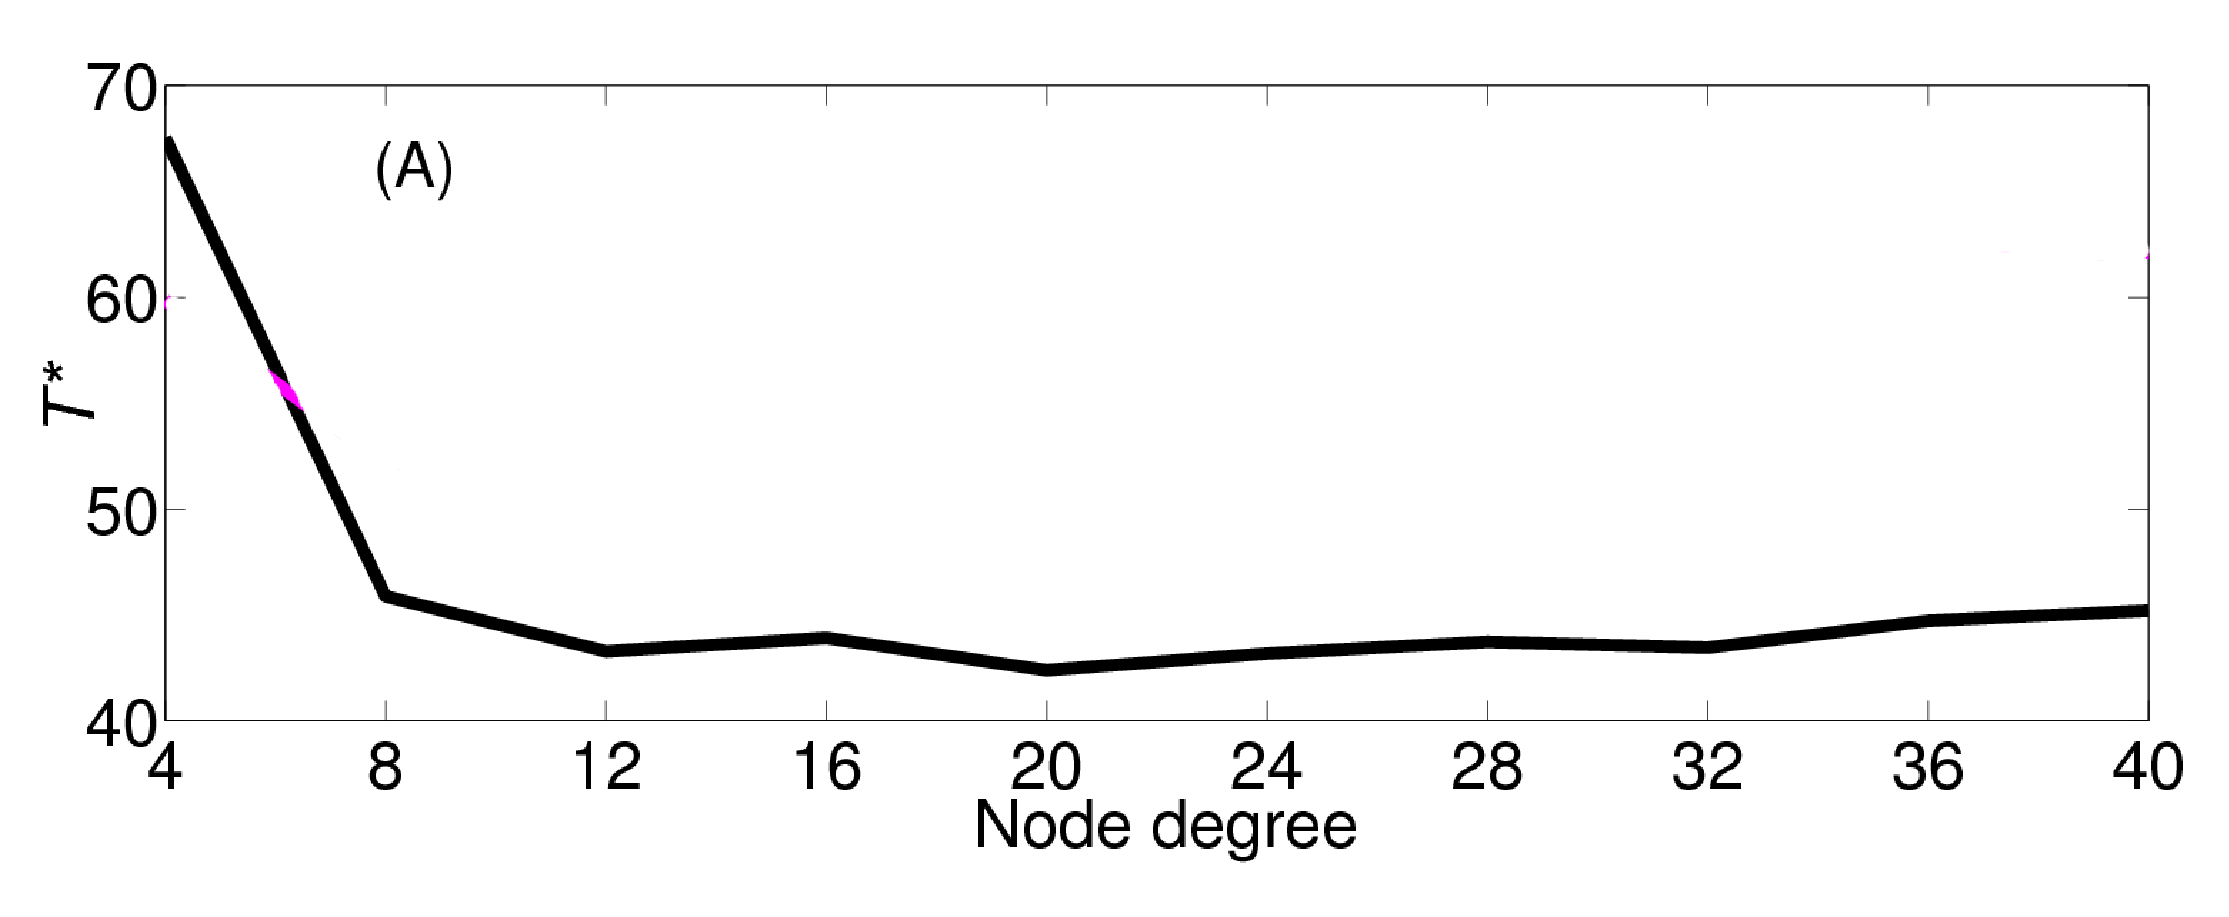
\includegraphics[scale=0.19]{./texfiles/Chapter_3/netsci/figs1/random_graphs_delay1.eps}
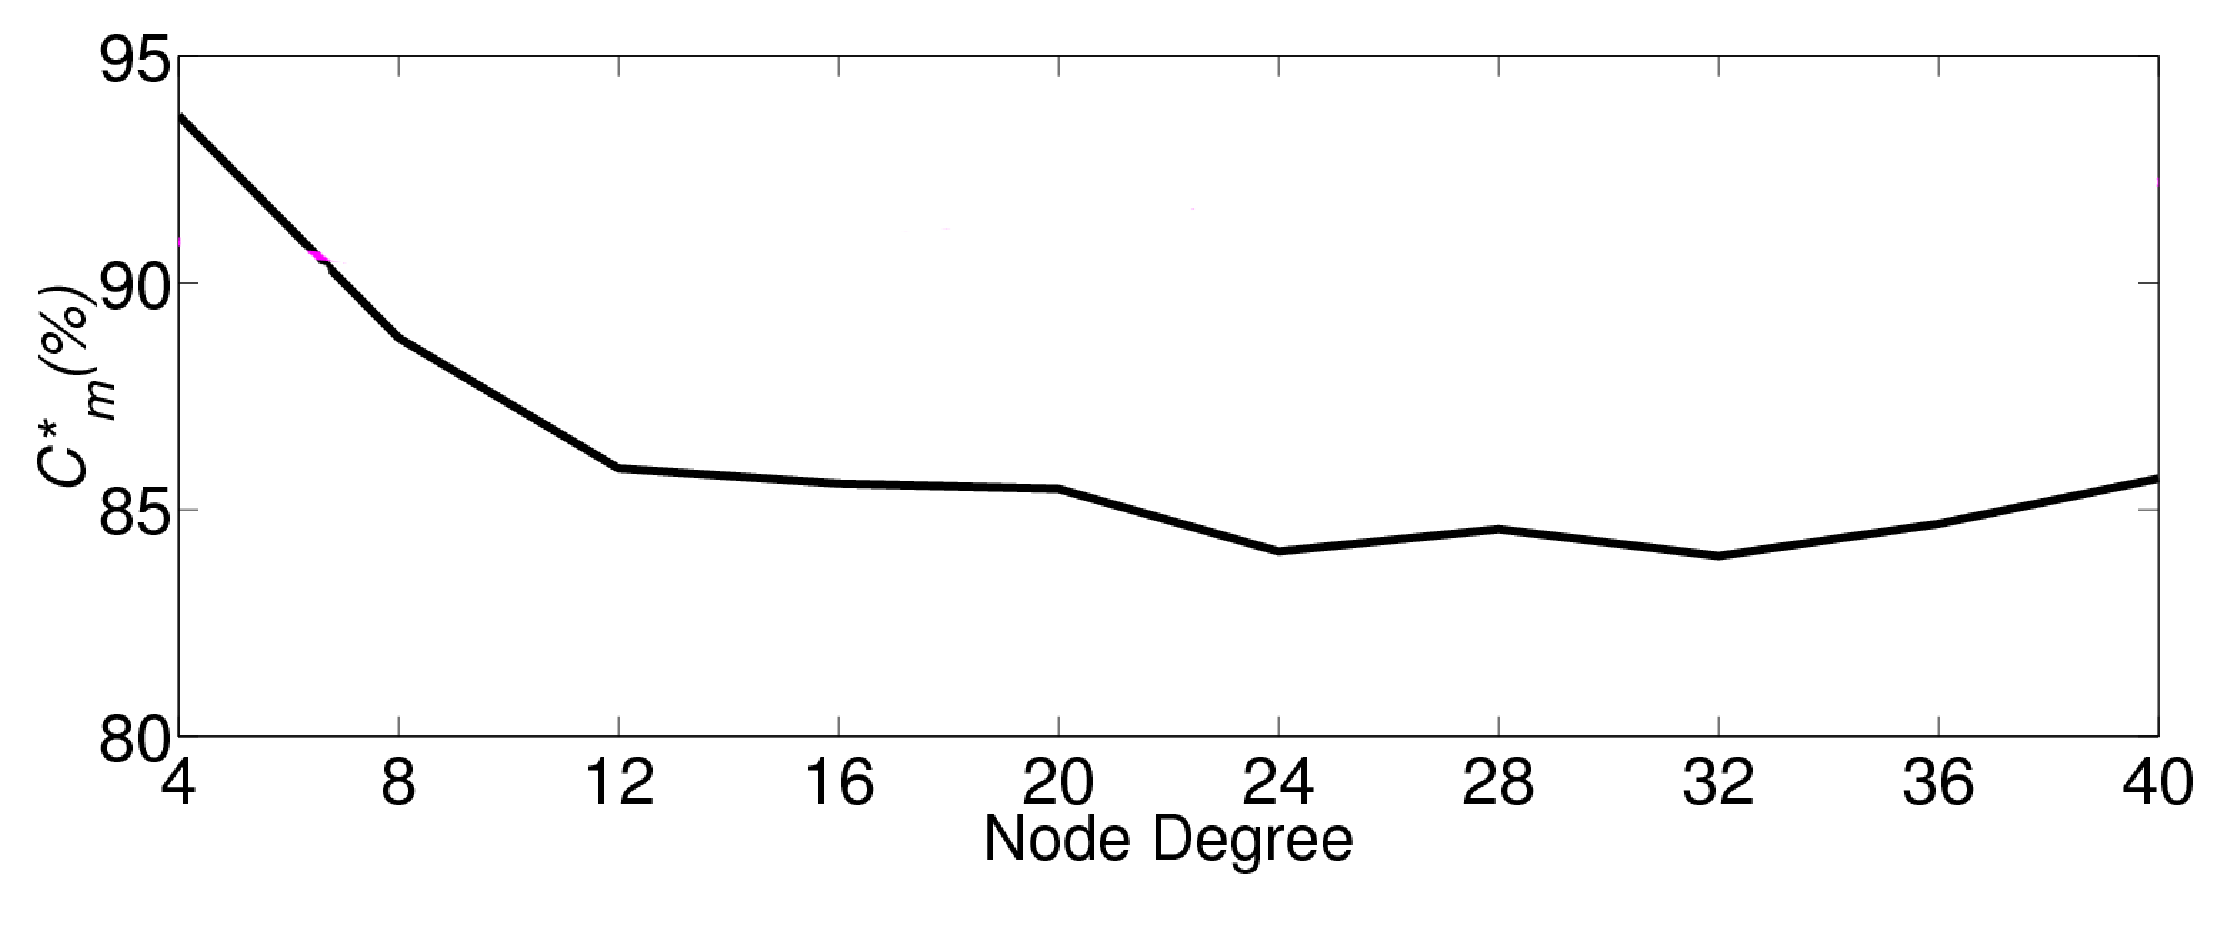
\includegraphics[scale=0.18]{./texfiles/Chapter_3/netsci/figs1/random_graphs_wastage1.eps}
\caption{(A) Broadcast time and (B) broadcast wastage versus average degree for B-P. The parameters values are $n=200, m=4, k=2$.\vspace{4mm}}
\label{DiffTopologyGnp_N200_varyD_push_pull}
\end{figure}
\begin{figure}
\centering
\includegraphics[scale=0.19]{./texfiles/Chapter_3/netsci/figs1/xperbt.eps}
\includegraphics[scale=0.19]{./texfiles/Chapter_3/netsci/figs1/xperwa.eps}
\caption{Average broadcast time and wastage versus $x$ for gnutella1, gnutella2 and gnutella3}
\label{ps_bt}
\end{figure}


\begin{figure*}[!ht]
  \centering	
 \includegraphics*[width=0.65\textwidth,height=40mm,angle=0]{./texfiles/Chapter_3/netsci/figs1/gnutella25_bt_wa_co.eps}
%\vspace{-5mm}
 
 \caption{\label{gnutellacomp} (A) Broadcast time versus message size (B) Wastage versus message size (C) Coverage versus message size for gnutella3}
\end{figure*}


\begin{figure*}[!ht]
  \centering	
 \includegraphics*[width=0.45\textwidth,height=40mm,angle=0]{./texfiles/Chapter_3/netsci/figs1/comp_gnut_4.eps}
 \includegraphics*[width=0.45\textwidth,height=40mm,angle=0]{./texfiles/Chapter_3/netsci/figs1/comp_gnut_6.eps}
%\vspace{-5mm}
 
 \caption{\label{gnutellacomp1} Gain in broadcast time of P-P-G over X-P-P and B-P [Inset shows gain in wastage] for (A) gnutella1 and (B) gnutella2 networks. Note: algo = B-P/X-P-P }
\vspace{.5cm}
 \end{figure*}
% \begin{figure*}[!ht]
%   \centering	
%  \includegraphics*[width=0.65\textwidth,height=40mm,angle=0]{figs1/gnutella25_bt_wa_co.eps}
% \vspace{-5mm}
%  
%  \caption{\label{gnutellacomp} (A) Broadcast time versus message size (B) Wastage versus message size (C) Coverage versus message size for gnutella1, gnutella2 and gnutella3\vspace{-3mm}}
% \end{figure*}

We measure 
the performance of the algorithms (B-P, X-P-P and P-P-G) on three real network traces based on broadcast time, 
wastage and coverage. The data sets are Gnutella network snapshots namely 
p2p-Gnutella04 (gnutella1), p2p-Gnutella06 (gnutella2) and p2p-Gnutella25 (gnutella3)~\cite{leskovec2007graph,ripeanu2002mapping} taken on dates August 4, August 6 and August 25, 2002 respectively. 
The gnutella1 network has 10876 nodes and 39994 edges in its largest connected component. Corresponding number of nodes and edges in the largest connected component 
in gnutella2 and gnutella3 are respectively 8717, 31525 and 22663, 54693. We simulate these algorithms for varying message sizes.
We perform our simulations on peer-to-peer systems specifically as our study can find a major application in such systems.

For simulating the X-P-P algorithm in particular we first need to obtain the best value of $x$ for each network and then run the simulations for varying message sizes. 
 In figure~\ref{ps_bt}, we show how the broadcast time and wastage varies with $x$ for networks gnutella1, gnutella2 and gnutella3. We observe that the best value of $x$ lies around 
 50\% for the gnutella1 network. Similarly the obtained value of $x$ are found to be around 50\% and 60\% for gnutella2 and gnutella3 
 respectively.
% We measure the performance of the three algorithms (B-P, P-G and P-P-G) on three real network traces based on broadcast time, 
% wastage and coverage. The data sets are Gnutella snapshots namely 
% p2p-Gnutella04 (gnutella1), p2p-Gnutella06 (gnutella2) and p2p-Gnutella25 ~\cite{ripeanu2002mapping,leskovec2007graph} taken on dates August 4, August 6 and August 25, 2002 respectively. 
% The gnutella1 network has 10876 nodes and 39994 edges in its largest connected component. Corresponding number of nodes and edges in the largest connected component 
% in gnutella2 and gnutella3 are respectively 8717, 31525 and 22663, 54693. We simulate these algorithms for varying message sizes.
% 
% For simulating the X-P-P algorithm we first obtain the best value of x for each network and then run the simulations for varying message sizes. 
%  In figure ~\ref{ss} and ~\ref{}, we show how the broadcast time and wastage varies with x for gnutella1 network. We obsreve that the best value of x lies around 
%  50\%. Similarly we obtained the value of x for the other two datasets as well and found it to be around 50\% and 60\% for gnutella2 and gnutella3 
%  respectively.
% As mentioned earlier we observe from simulation results (shown in figure [4]) that the P-G algorithm performs better than B-P with respect to broadcast time and 
%  wastage with a reasonably good coverage of around 95\% when message size is 2. However, the coverage drastically falls as we increase the message size. 
%  P-P-G performs best among all the algorithms in terms of broadcast time.
%  It is so because the non-sender nodes are allowed $pull$ opportunities in addition to $push$ by 
%  sender nodes. In addition, it can be noticed that the overall wastage with respect to B-P is also reduced significantly. 
%  X-P-P performs best in terms of wastage and is second only to P-P-G in terms of broadcast time. Actually, X-P-P provides the best optimization 
%   between broadcast time and wastage but would incur significant computational overhead if implemented; in fact, it is infeasible in practical distributed settings.
%  Note that it is almost impossible to have an algorithm which optimizes both broadcast time and wastage yet providing maximum coverage.
%  Our proposed algorithm (P-P-G) presents the best possible trade-off of delay and wastage guaranteeing almost 100\% coverage and can be 
%  implemented in a distributed fashion with almost negligible computational overhead.
In figure ~\ref{gnutellacomp} we plot the broadcast time, wastage and coverage for gnutella3 network. 
We observe that with P-P-G we gain in both broadcast time and wastage with respect to B-P. With respect to X-P-P, P-P-G offers better 
broadcast time but with a higher wastage.
For gnutella1 and gnutella2 networks 
we plot (figure ~\ref{gnutellacomp1}) the ratio of broadcast time and wastage of X-P-P and B-P over P-P-G for different message sizes. 
% We observe that accross different message sizes on an average the ratio of broadcast time of X-P-P over P-P-G is around $1.5$ and that for B-P over P-P-G is $5.8$. 
% The corresponding values for wastage are $0.75$ and $1.10$ respectively. 
We observe that across different message sizes, on average the increase in broadcast time of X-P-P over P-P-G and B-P over P-P-G are $5.45$ and $1.5$ respectively for 
gnutella1 network while for gnutella2 network the corresponding values are 5.9 and 1.6 respectively. Corresponding values for wastage are $0.75$ and $1.10$ 
respectively for gnutella1 network and $0.72$ and $1.06$ respectively for gnutella2 network. 
So with P-P-G we gain in both broadcast time and wastage with respect to B-P while with respect to X-P-P 
we gain in broadcast time without significant increase in wastage.
 Actually, X-P-P provides the best optimization between broadcast time and wastage but it would be hard to implement in a 
distributed setting. 
Our proposed algorithm (P-P-G) presents the best possible trade-off between delay and wastage guaranteeing almost 100\% coverage and can be implemented in a distributed fashion with almost negligible computational overhead.
% \begin{figure*}[!ht]
%   \centering
%   \includegraphics*[width=0.65\textwidth,height=40mm,angle=0]{figs1/gnutella4_bt_wa_co.eps}
% 
%  \vspace{-5mm}
%  %\caption{\label{gnutellacomp} (A) broadcast time versus message size (B) wastage versus message size (C) coverage versus message size for gnutella1, gnutella2 and gnutella3}
% \end{figure*}
% \begin{figure*}[!ht]
%   \centering
%  \includegraphics*[width=0.65\textwidth,height=40mm,angle=0]{figs1/gnutella6_bt_wa_co.eps}	
%  \vspace{-5mm}
% 
%  
%  %\caption{\label{gnutellacomp} (A) broadcast time versus message size (B) wastage versus message size (C) coverage versus message size for gnutella1, gnutella2 and gnutella3}
% \end{figure*}
% 
% \begin{figure*}[!ht]
%   \centering	
%  \includegraphics*[width=0.45\textwidth,height=40mm,angle=0]{figs1/comp_gnut_4.eps}
%  \includegraphics*[width=0.45\textwidth,height=40mm,angle=0]{figs1/comp_gnut_6.eps}
% \vspace{-5mm}
%  
%  \caption{\label{gnutellacomp1} Efficiency in broadcast time of P-P-G over X-P-P and B-P for gnutella1 and gnutella2 networks. (inset) efficiency in wastage of P-P-G over X-P-P and P-G \vspace{-10mm}}
% \end{figure*}
% We measure the performance of the three algorithms (B-P, P-G and P-P-G) on three real network traces based on broadcast time, 
% wastage and coverage. The data sets are Gnutella snapshots namely 
% p2p-Gnutella04 (gnutella1), p2p-Gnutella06 (gnutella2) and p2p-Gnutella25 ~\cite{ripeanu2002mapping,leskovec2007graph} taken on dates August 4, August 6 and August 25, 2002 respectively. 
% The gnutella1 network has 10876 nodes and 39994 edges in its largest connected component. Corresponding number of nodes and edges in the largest connected component 
% in gnutella2 and gnutella3 are respectively 8717, 31525 and 22663, 54693. We simulate these algorithms for varying message sizes.

% \begin{figure*}[!ht]
%   \centering
%   \includegraphics*[width=0.7\textwidth,height=55mm,angle=0]{figs1/gnutella4_bt_wa_co.eps}
% 
%  \vspace{-5mm}
%  %\caption{\label{gnutellacomp} (A) broadcast time versus message size (B) wastage versus message size (C) coverage versus message size for gnutella1, gnutella2 and gnutella3}
% \end{figure*}
% \begin{figure*}[!ht]
%   \centering
%  \includegraphics*[width=0.7\textwidth,height=55mm,angle=0]{figs1/gnutella6_bt_wa_co.eps}	
%  \vspace{-5mm}
% 
%  
%  %\caption{\label{gnutellacomp} (A) broadcast time versus message size (B) wastage versus message size (C) coverage versus message size for gnutella1, gnutella2 and gnutella3}
% \end{figure*}
% \begin{figure*}[!ht]
%   \centering	
%  \includegraphics*[width=0.7\textwidth,height=55mm,angle=0]{figs1/gnutella25_bt_wa_co.eps}
% \vspace{-5mm}
%  
%  \caption{\label{gnutellacomp} (A) broadcast time versus message size (B) wastage versus message size (C) coverage versus message size for gnutella1, gnutella2 and gnutella3}
% \end{figure*}
%  \begin{figure}
% \centering
% 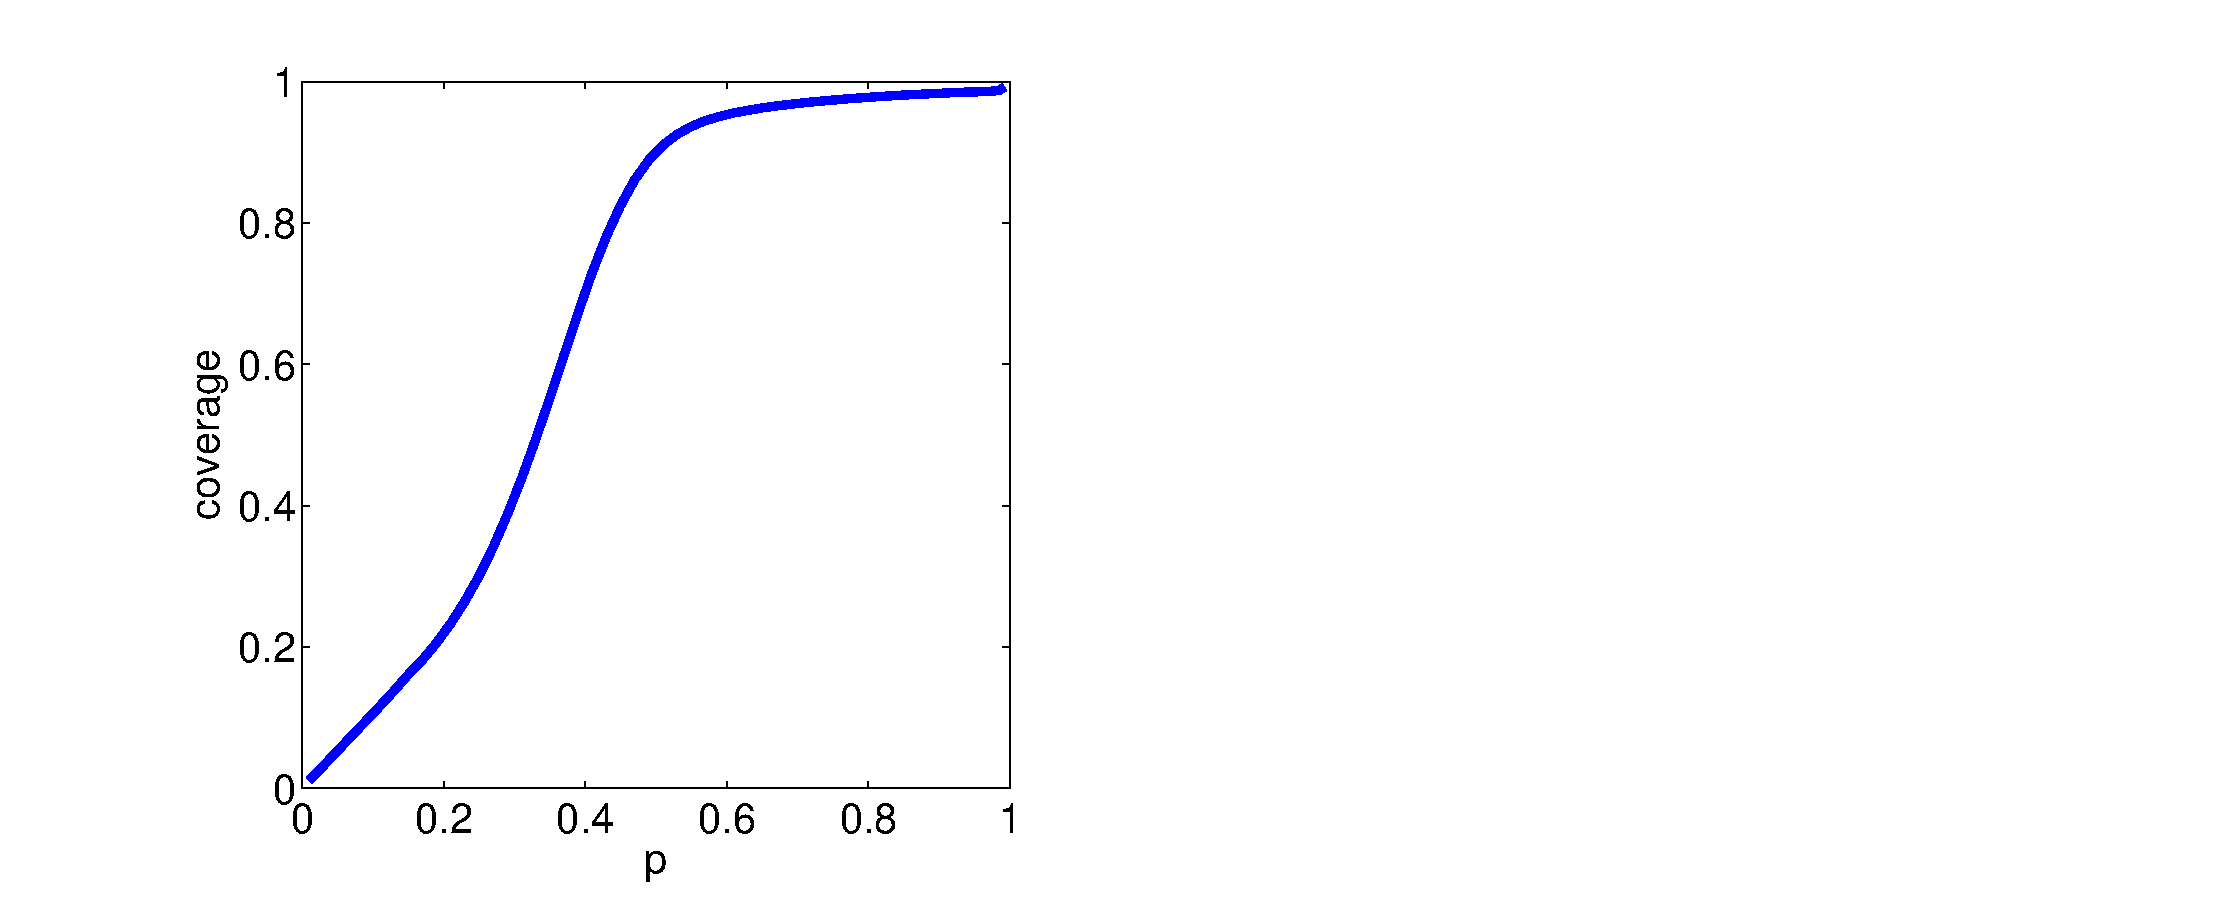
\includegraphics[scale=0.4]{figs1/pvsco.eps}
% \caption{(A) Broadcast time and (B) broadcast wastage versus different values of $d$ for B-P. The parameters values are $n=200, m=4, k=2$.\vspace{-3mm}}
% \label{pcov}
% \end{figure}
%  For simulating the X-P-P algorithm we first obtain the best value of x for each network and then run the simulations for varying message sizes. 
%  In figure ~\ref{ss} and ~\ref{}, we show how the broadcast time and wastage varies with x for gnutella1 network. We obsreve that the best value of x lies around 
%  50\%. Similarly we obtained the value of x for the other two datasets as well and found it to be around 50\% and 60\% for gnutella2 and gnutella3 
%  respectively.
 
%  As mentioned earlier we observe from simulation results (shown in figure [4]) that the P-G algorithm performs better than B-P with respect to broadcast time and 
%  wastage with a reasonably good coverage of around 95\% when message size is 2. However, the coverage drastically falls as we increase the message size. 
%  P-P-G performs best among all the algorithms in terms of broadcast time.
%  It is so because the non-sender nodes are allowed $pull$ opportunities in addition to $push$ by 
%  sender nodes. In addition, it can be noticed that the overall wastage with respect to B-P is also reduced significantly. 
%  X-P-P performs best in terms of wastage and is second only to P-P-G in terms of broadcast time. Actually, X-P-P provides the best optimization 
%   between broadcast time and wastage but would incur significant computational overhead if implemented; in fact, it is infeasible in practical distributed settings.
%  Note that it is almost impossible to have an algorithm which optimizes both broadcast time and wastage yet providing maximum coverage.
%  Our proposed algorithm (P-P-G) presents the best possible trade-off of delay and wastage guaranteeing almost 100\% coverage and can be 
%  implemented in a distributed fashion with almost negligible computational overhead.
%  We also mentioned previously that the condition for give-up has a factor $p$ 
%  (we consider the threshold for give-up to be $f*(|l_{i}|+1)$ and $f=-\log(1-p)$) through which we can control the coverage. 
%  In figure [5] we plot the value of $p$ versus coverage for gnutella1 network. We observe that the coverage increases gradually as we 
%  increase $p$. So, for a greater coverage one needs to use a sufficiently large value of $p$ and vice-versa. 
%  We show this effect only empirically in this 
%  paper but we plan to analyze it in more details analytically in a forthcoming paper.
% \begin{figure}
% \centering
% 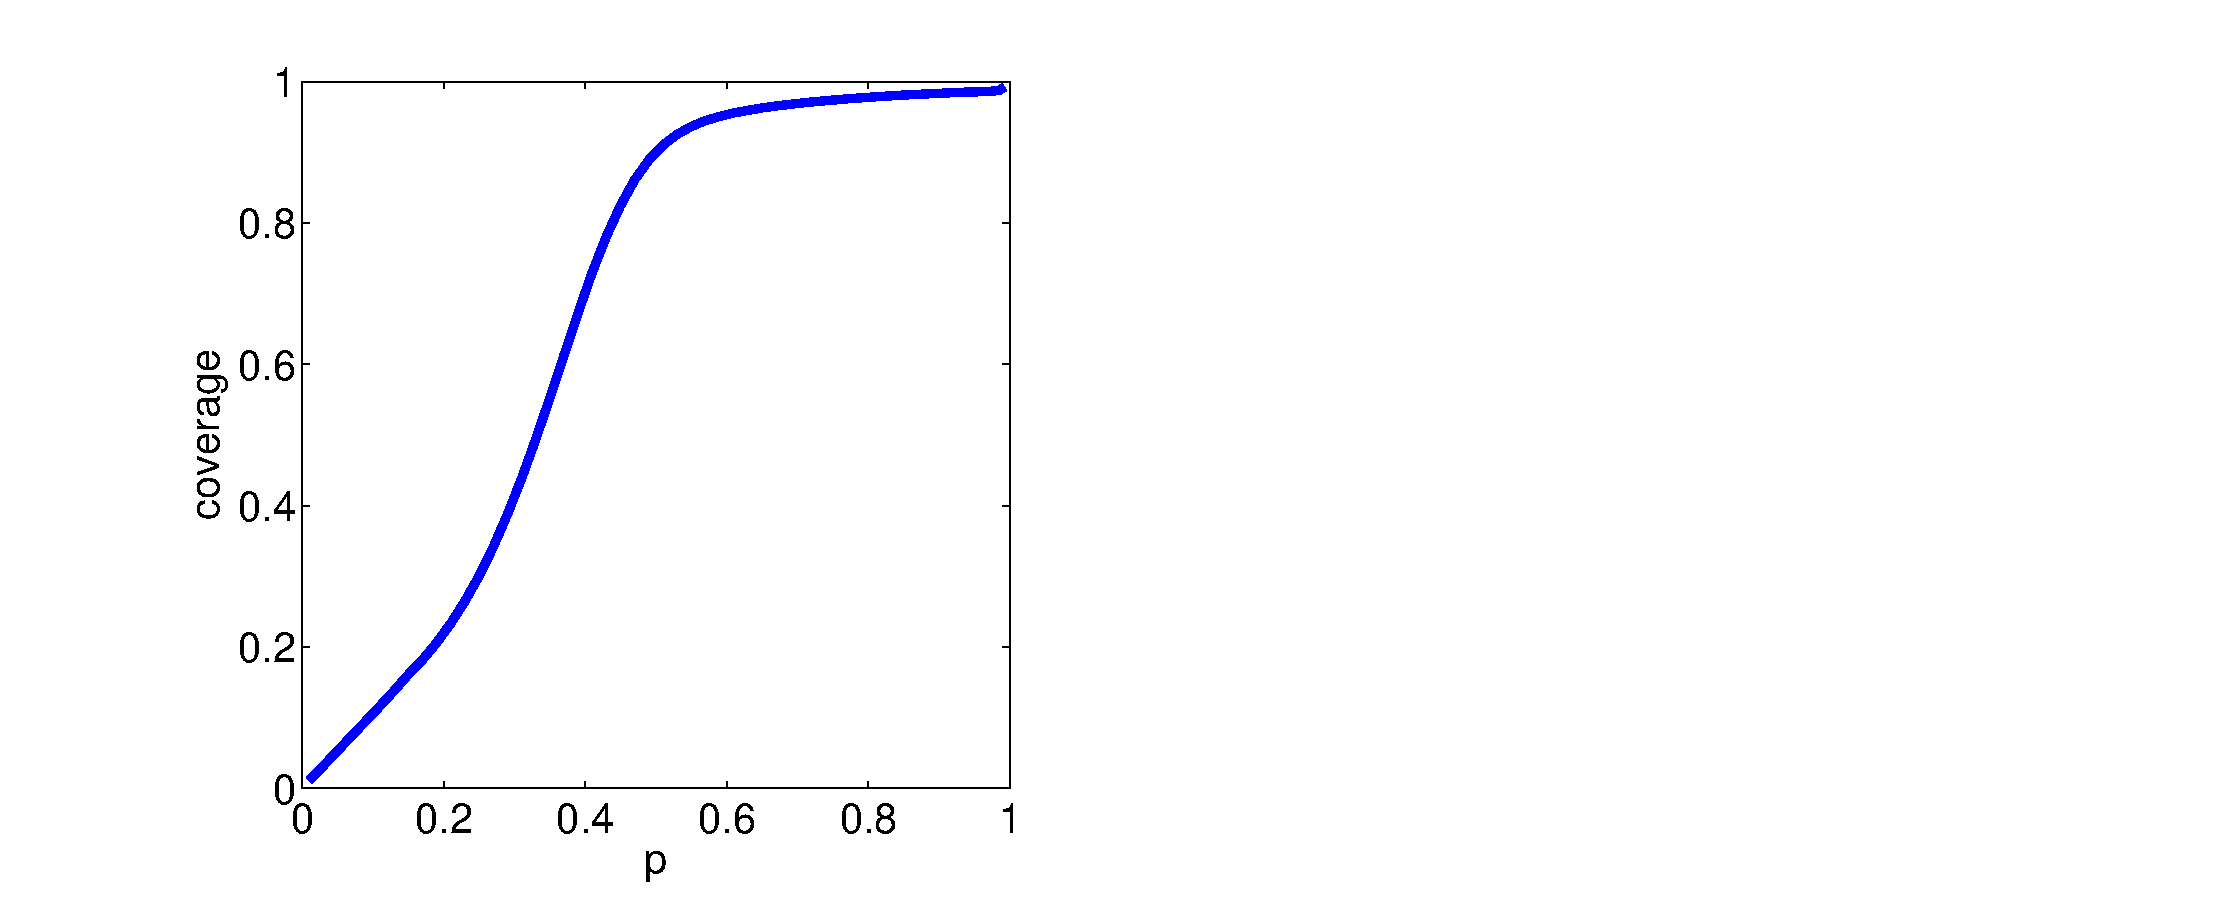
\includegraphics[scale=0.4]{figs1/pvsco.eps}
% \caption{$p$ versus coverage for gnutella1 network\vspace{-3mm}}
% \label{pcov}
% \end{figure}
%\vspace{-2mm}
\subsubsection{Effect of degree on broadcast time}

  In earlier part of this section we observed that irrespective of the topology one is able to  
obtain a critical value of $d$ for which the 
  broadcast time is minimum. So we perform simulations on sparser variants of these gnutella networks
and observe that broadcast time reduces even for the B-P. To obtain sparser variants, we consider each gnutella snapshot and randomly removed 
some of the edges 
without hampering the network connectivity. From figure ~\ref{gnutellasparse} we observe that the broadcast time reduces significantly
in case of the sparser variants in comparison to the original network.
Hence, while designing a network it is advisable to keep the network sparse rather than creating unnecessary connections between the nodes.
This, as our results indicate, should lead to a faster dissemination of messages.


% Since the value of the critical average degree is found to be on the lower side, we performed simulations on sparser variants of the real traces (used previously)
% and observed that broadcast time reduces even for the B-P. We considered each gnutella snapshot and randomly removed some of the edges such that the
% network remains connected while producing a sparser variant. From figure ~\ref{gnutellasparse} we observe that the broadcast time reduces significantly
% in case of the sparser variants in comparison to the original network.
% Hence, while designing a network it is advisable to keep the network sparse rather than creating unnecessary connections between the nodes.
% This, as our results indicate, should lead to a faster dissemination of messages.

\begin{figure}
\centering
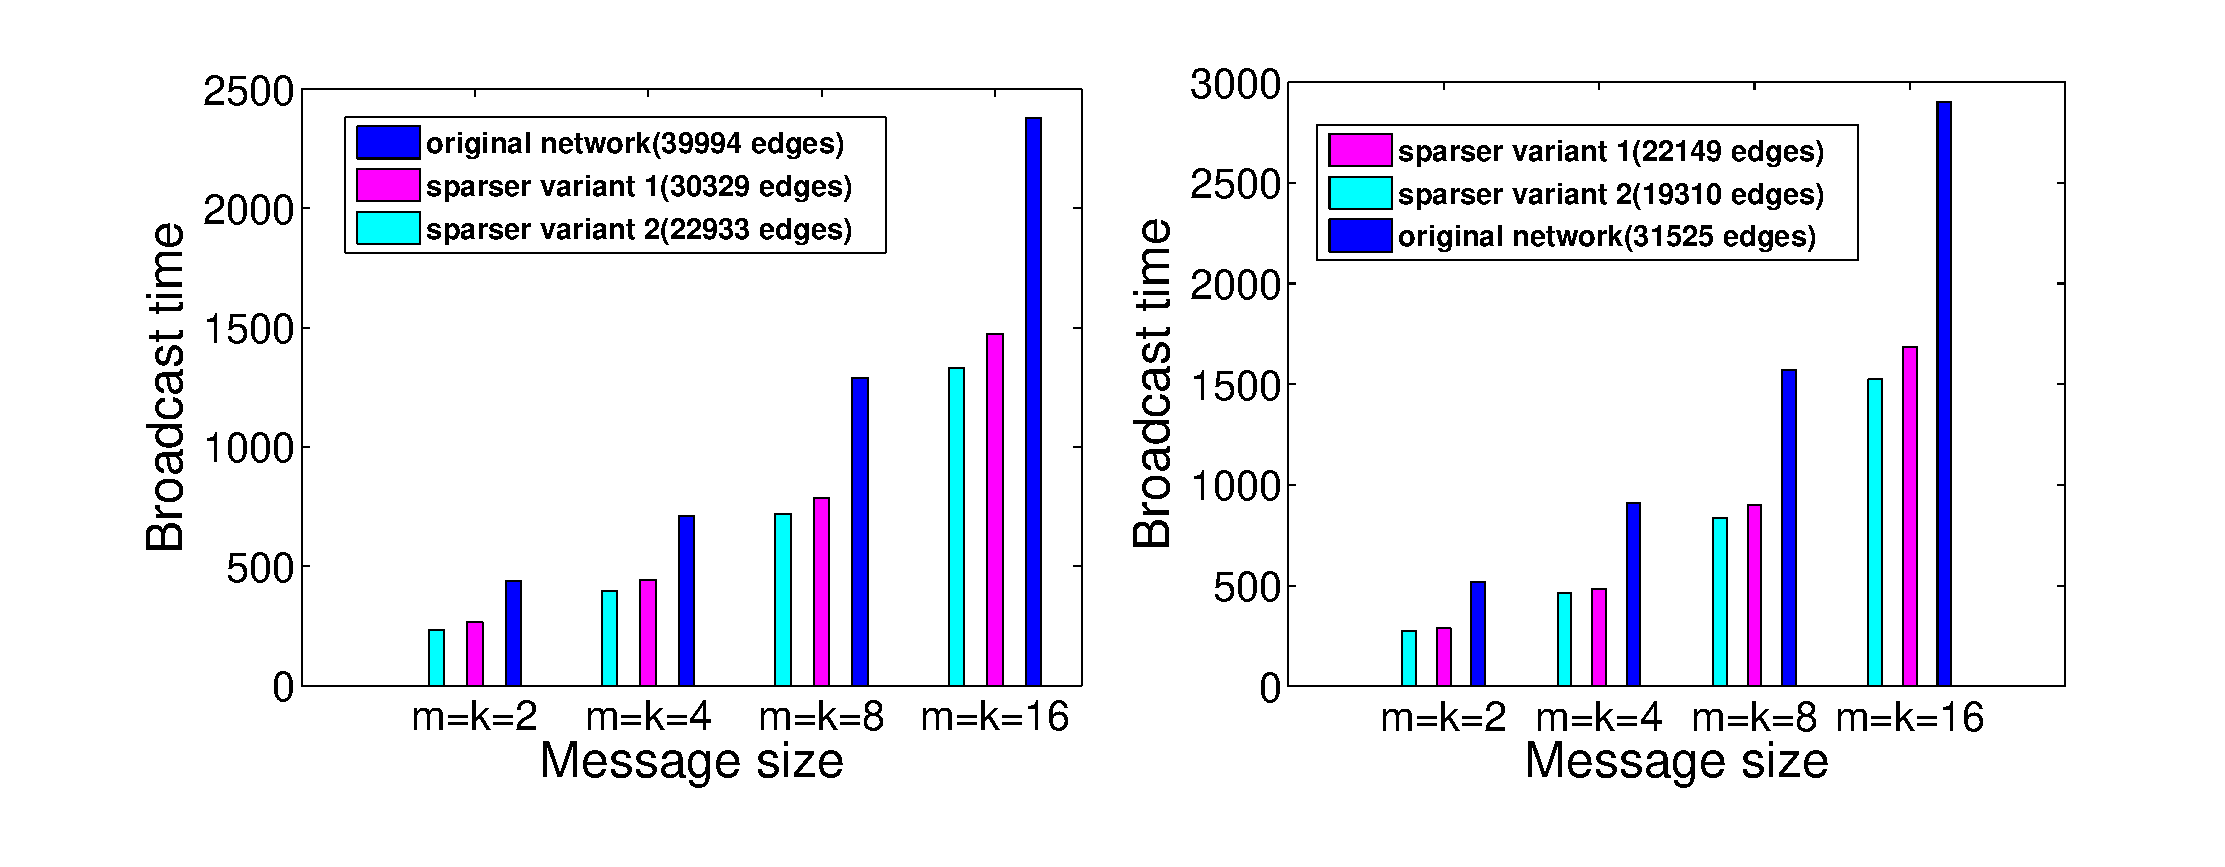
\includegraphics[scale=0.25]{./texfiles/Chapter_3/netsci/figs1/gnutella1_gnutella2.eps}
%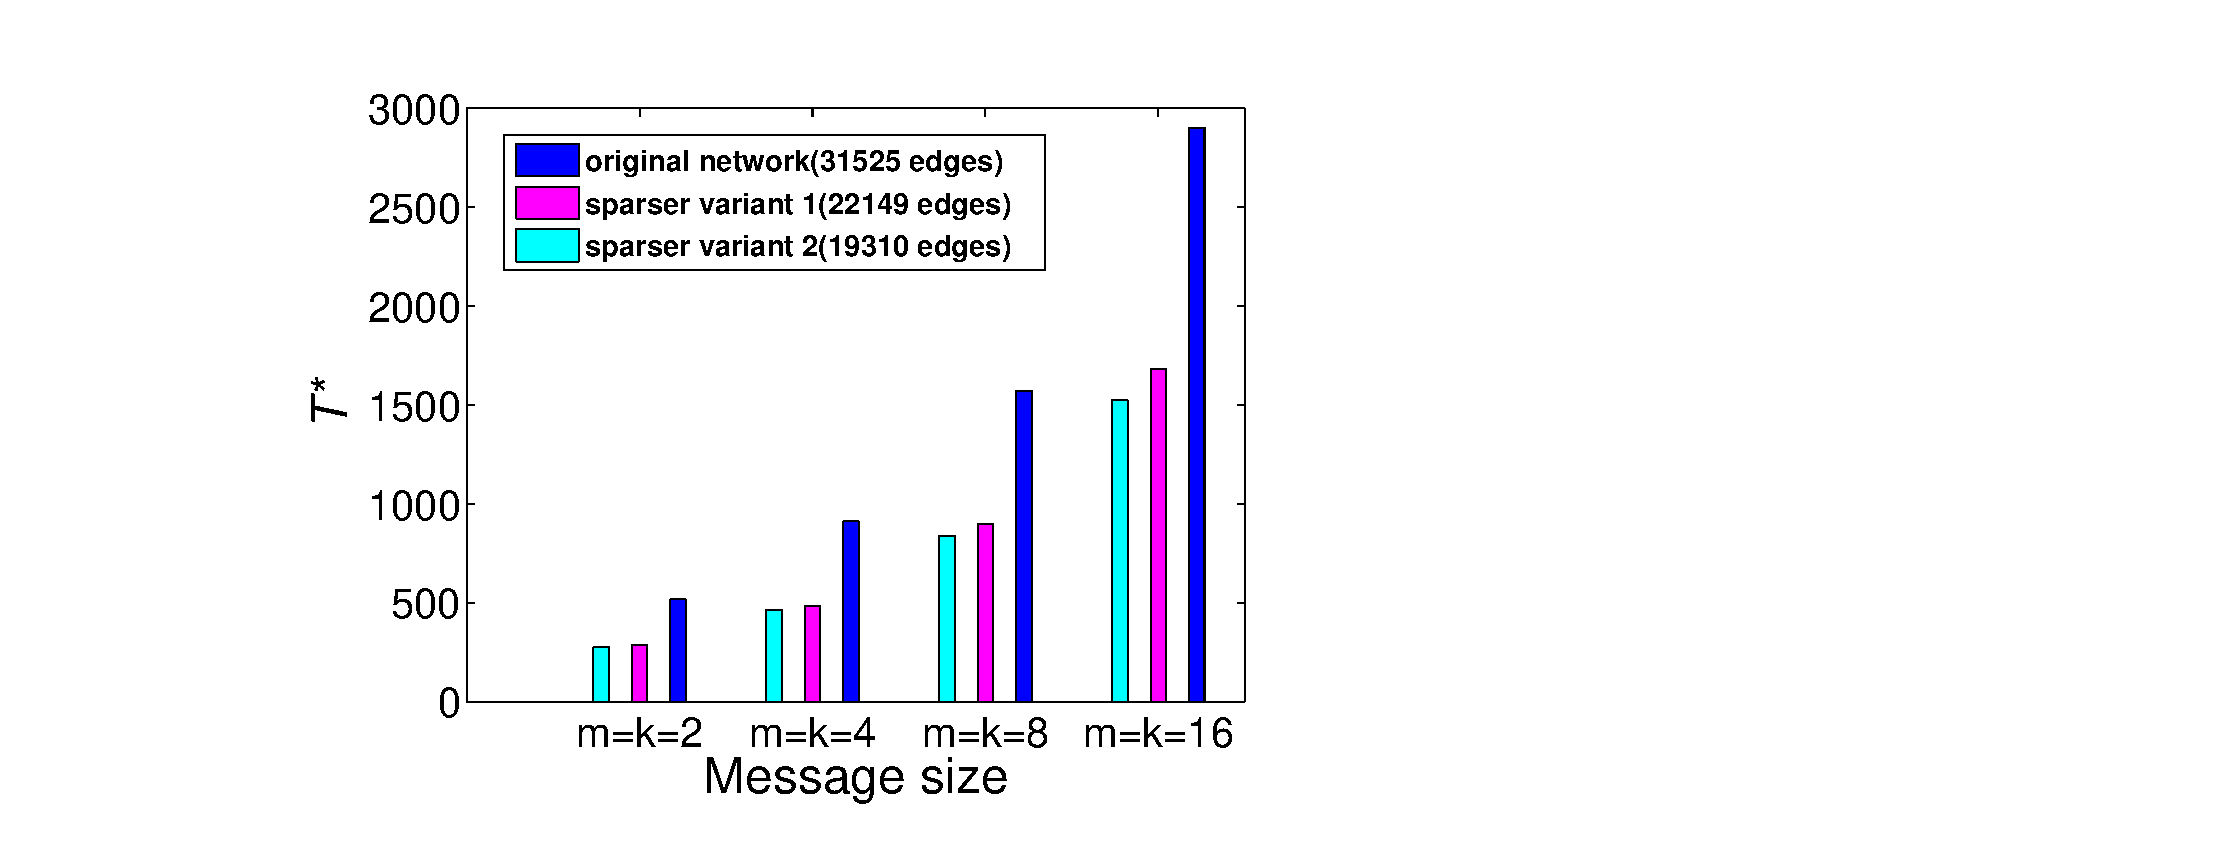
\includegraphics[scale=0.25]{figs1/gnutella2.eps}
%\vspace{-8mm}
\caption{Broadcast time for the gnutella snapshots and their sparser variants versus different values of message sizes for (a). gnutella1 and (b). gnutella2}
\label{gnutellasparse}
\vspace{.5cm}
\end{figure}
\medskip

 \medskip
